\documentclass[11pt,a4paper]{article}
%-------------------------------------------
%---Packages--------------------------------
%-------------------------------------------
\usepackage[utf8]{inputenc}
%\usepackage[T1]{fontenc}
%\usepackage{txfonts}
\usepackage{amsmath}
\usepackage{amsthm}
\usepackage{amsfonts}
\usepackage{array}
\usepackage{amssymb}
\usepackage{blindtext}
\usepackage{caption}
\usepackage{color}
\usepackage{csquotes}	    %
\usepackage{enumitem}	    %pour mieux bosser avec les listes. ajoute option label
\usepackage[yyyymmdd]{datetime}        %pour définir date custom
\usepackage{etaremune}
\usepackage{environ}
\usepackage{fancybox}
\usepackage{fancyhdr} 	    % Custom headers and footers
\usepackage{fancyref}
%\usepackage{float}
\usepackage{floatrow}       %float and floatrow can't be together...
\usepackage{gensymb}
\usepackage{graphicx}
\usepackage[colorlinks=true, linkcolor=purple, citecolor=cyan]{hyperref}
\usepackage{footnotebackref}
\usepackage{lipsum}
\usepackage{mathtools}
\usepackage{multicol}	    %gérer plusieurs colonnes
\usepackage{setspace}
\usepackage{subcaption}
\usepackage{todonotes}	    %Bonne gestion des TODOs
%TODO commenté pour tester l'utilité... à voir% \usepackage[tc]{titlepic}      %Permet de mettre une image en page de garde
\usepackage{tikz}	    % Pour outil de dessin puissant
\usepackage{ulem}	    %underline sur plusieurs lignes (avec \uline{})
\usepackage{vmargin} 	    %gestion des marges, avec dans l'ordre : gauche, haut, droit, bas, en-tête, entre en-tête et texte, bas de page, hauteur entre bas de page et texte
\usepackage{wrapfig}
\usepackage{xcolor}
\usepackage{xparse}                    %Pour utiliser NewDocumentCommand et des arguments 'mmooo'
%\usepackage{fullpage} 	    %supprime toutes les marges allouées aux notes, aussi en haut et en bas

%\ExplSyntaxOn
\pagestyle{fancyplain}	    %Makes all pages in the document conform to the custom headers and footers

%-------------------------------------------
%---Document Commands-----------------------
%---------------------------{----------------
\NewDocumentCommand{\framecolorbox}{oommm}
 {% #1 = width (optional)
  % #2 = inner alignment (optional)
  % #3 = frame color
  % #4 = background color
  % #5 = text
  \IfValueTF{#1}%
   {\IfValueTF{#2}%
    {\fcolorbox{#3}{#4}{\makebox[#1][#2]{#5}}}%
    {\fcolorbox{#3}{#4}{\makebox[#1]{#5}}}%
   }%
   {\fcolorbox{#3}{#4}{#5}}%
 }%
%------------------------------------------------
%------------------ENGLISH----------------------
%----------------------------------------------

\NewDocumentCommand{\epflTitle}{mO{Olivier Cloux}O{\today}O{Notes de Cours en}D<>{../../Common}}%Arguments : Matière, Auteur, Date, Titre du doc
{
\begin{titlepage}
    \vspace*{\fill}
    \begin{center}
        \normalfont \normalsize
        \textsc{Ecole Polytechnique Fédérale de Lausanne} \\ [25pt] % Your university, school and/or department name(s)
        \textsc{#4} %Titre du doc
        \\ [0.4 pt]
        \horrule{0.5pt} \\[0.4cm] % Thin top horizontal rule
        \huge #1 \\ % Matière
        \horrule{2pt} \\[0.5cm] % Thick bottom horizontal rule
        
\includegraphics[width=8cm]{#5/EPFL_logo}
        ~\\[0.5 cm]
        \small\textsc{#2}\\[0.4cm]
        \small\textsc{#3}\\
        ~\\
        ~\\
        
\includegraphics[scale=0.5]{#5/creativeCommons}
    \end{center}
    \vspace*{\fill}
\end{titlepage}
}


%-------------------------------------------
%-------------MATH NEW COMMANDS-------------
%-------------------------------------------
\newcommand{\somme}[2]{\ensuremath{\sum\limits_{#2}^{#1}}}
\newcommand{\produit}[2]{\ensuremath{\prod\limits_{#2}^{#1}}}
\newcommand{\limite}{\lim\limits_}
\newcommand{\llimite}[3]{\limite{\substack{#1 \\ #2}}\left(#3\right)}	%limites à deux condiitons
\newcommand{\et}{\mbox{ et }}
\newcommand{\deriv}[1]{\ensuremath{\, \mathrm d #1}}	%sigle dx, dt,dy... des dérivées/intégrales
%\newcommand{\fx}{\ensuremath{f'(\textbf{x}_0 + h}}
\newcommand{\ninf}{\ensuremath{n \to \infty}}	       %pour les limites : n tend vers l'infini
\newcommand{\xinf}{\ensuremath{x \to \infty}}	       %pour les limites : x tend vers l'infini
\newcommand{\infint}{\ensuremath{\int_{-\infty}^{\infty}}}
\newcommand{\xo}{\ensuremath{x \to 0}}									%x to 0
\newcommand{\no}{\ensuremath{n \to 0}}									%n zéro
\newcommand{\xx}{\ensuremath{x \to x}}									%x to x
\newcommand{\Xo}{\ensuremath{x_0}}										%x zéro
\newcommand{\X}{\ensuremath{\mathbf{X}} }
\newcommand{\A}{\ensuremath{\mathbf{A}} }
\newcommand{\R}{\ensuremath{\mathbb{R}} }								%ensemble de R
\newcommand{\rn}{\ensuremath{\mathbb{R}^n} } 							%ensemble de R de taille n
\newcommand{\Rm}{\ensuremath{\mathbb{R}^m} }  							%ensemble de R de taille m
\newcommand{\C}{\ensuremath{\mathbb{C}} }
\newcommand{\N}{\ensuremath{\mathbb{N}} }
\newcommand{\Z}{\ensuremath{\mathbb{Z}} }
\newcommand{\Q}{\ensuremath{\mathbb{Q}} }
\newcommand{\rtor}{\ensuremath{\R \to \R} }
\newcommand{\pour}{\mbox{ pour }}
\newcommand{\coss}[1]{\ensuremath{\cos\(#1\)}}						%cosinus avec des parenthèses de bonne taille (genre frac)
\newcommand{\sinn}[1]{\ensuremath{\sin\(#1\)}}					%sinus avec des parentèses de bonne taille (genre frac)
\newcommand{\txtfrac}[2]{\ensuremath{\frac{\text{#1}}{\text{#2}}}}		%Fractions composées de texte
\newcommand{\evalfrac}[3]{\ensuremath{\left.\frac{#1}{#2}\right|_{#3}}}
\renewcommand{\(}{\left(}												%Parenthèse gauche de taille adaptive
\renewcommand{\)}{\right)}
\newcommand{\longeq}{=\joinrel=}												%Parenthèse droite de taille adaptive


%-------------------------------------------------------
%------------------MISC NEW COMMANDS--------------------
%-------------------------------------------------------
\newcommand{\degre}{\ensuremath{^\circ}}
%\newdateformat{\eudate}{\THEYEAR-\twodigit{\THEMONTH}-\twodigit{\THEDAY}}



%-------------------------------------------------------
%------------------TEXT NEW COMMANDS--------------------
%-------------------------------------------------------
\newcommand{\ts}{\textsuperscript}
\newcommand{\evid}[1]{\textbf{\uline{#1}}}        %mise en évidence (gras + souligné)



%\newcommand{\Exemple}{\underline{Exemple}}
\newcommand{\Theoreme}{\underline{Théorème}}
\newcommand{\Remarque}{\underline{Remarque}}
\newcommand{\Definition}{\underline{Définition} }
\newcommand{\skinf}{\sum^{\infty}_{k=0}}
\newcommand{\combi}[2]{\ensuremath{\begin{pmatrix} #1 \\ #2 \end{pmatrix}}}	%combinaison parmi 1 de 2
\newcommand{\intx}[3]{\ensuremath{\int_{#1}^{#2} #3 \deriv{x}}}				%intégrale dx
\newcommand{\intt}[3]{\ensuremath{\int_{#1}^{#2} #3 \deriv{t}}}				%intégrale dy
\newcommand{\misenforme}{\begin{center} Mis en forme jusqu'ici\\ \line(1,0){400}\\ normalement juste, mais à améliorer depuis ici\end{center}}	%raccourci pour mise en forme
\newcommand*\circled[1]{\tikz[baseline=(char.base)]{
            \node[shape=circle,draw,inner sep=1pt] (char) {#1};}}			%pour entourer un chiffre
\newcommand{\horrule}[1]{\rule{\linewidth}{#1}} 				% Create horizontal rule command with 1 argument of height

\theoremstyle{definition}
\newtheorem{exemp}{Exemple}
\newtheorem{examp}{Example}


%-------------------------------------------
%---Environments----------------------------
%-------------------------------------------
\NewEnviron{boite}[1][0.9]{%
	\begin{center}
		\framecolorbox{red}{white}{%
			\begin{minipage}{#1\textwidth}
 	 			\BODY
			\end{minipage}
		}
	\end{center}
}
\NewEnviron{blackbox}[1][0.9]{%
	\begin{center}
		\framecolorbox{black}{white}{%
			\begin{minipage}{#1\textwidth}
 	 			\BODY
			\end{minipage}
		}
	\end{center}
}
\NewEnviron{exemple}[1][0.8]{%
    \begin{center}
        \framecolorbox{white}{gray!20}{%
            \begin{minipage}{#1\textwidth}
                \begin{exemp}
                    \BODY
                \end{exemp}
            \end{minipage}
        }
    \end{center}
}
\NewEnviron{suiteExemple}[1][0.8]{%
    \begin{center}
        \framecolorbox{white}{gray!20}{%
            \begin{minipage}{#1\textwidth}
                \BODY
            \end{minipage}
        }
    \end{center}
}
\NewEnviron{colExemple}[1][0.8]{%
    \begin{center}
        \framecolorbox{white}{gray!20}{%
            \begin{minipage}{#1\columnwidth}
                \begin{exemp}
                    \BODY
                \end{exemp}
            \end{minipage}
        }
    \end{center}
}
\NewEnviron{example}[1][0.8]{%
    \begin{center}
        \framecolorbox{white}{gray!20}{%
            \begin{minipage}{#1\textwidth}
                \begin{examp}
                    \BODY
                \end{examp}
            \end{minipage}
	}
    \end{center}
}
\NewEnviron{systeq}[1][l]{
			\begin{center}
				$\left\{\begin{array}{#1}
					\BODY
				\end{array}\right.$
			\end{center}
 }





%-------------------------------------------
%---General settings-----------------------
%-------------------------------------------
\renewcommand{\headrulewidth}{1pt}										%ligne au haut de chaque page
\renewcommand{\footrulewidth}{1pt}										%ligne au pied de chaque page
\setstretch{1.6}
\author{Olivier Cloux}

\begin{document}
\epflTitle{Signal Processing for Communications}[Olivier Cloux][Spring 2017][Summary in]<../../../Common/>
\setstretch{1.1}
\setlist[itemize]{font=\bfseries\uline, leftmargin=2cm}
\setlength{\abovedisplayskip}{0.1cm}
\setlength{\belowdisplayskip}{0.1cm}
\setlength{\multicolsep}{0pt}
\setlength{\columnsep}{-80pt}
\tableofcontents
\newpage
%%%%%%%%%%%%%%%%%%%%%%%%
%%%% Introduction %%%%%%
%%%%%%%%%%%%%%%%%%%%%%%%
\section{Introduction}
\begin{itemize}
    \setlength\itemsep{-0.2em}

    \item[Signals] Describe the evolution of a real life phenomenon.

    \item[Sampling] Instead of considering \textit{continuous} time signals (temperature,\ldots), it might be easier to \textbf{sample} them and consider it as \textit{discrete}
    
    \item[Sampling Theorem] See Figure~\ref{fig_sampling_theorem} and equation~\ref{equ_sampling_theorem}
        \begin{equation}
            x(t) = \somme{\infty}{n=-\infty} x[n] sinc\left(\frac{t-nT_s}{T_s}\right)%
            \label{equ_sampling_theorem}
        \end{equation}
        \begin{figure}
            \centering
            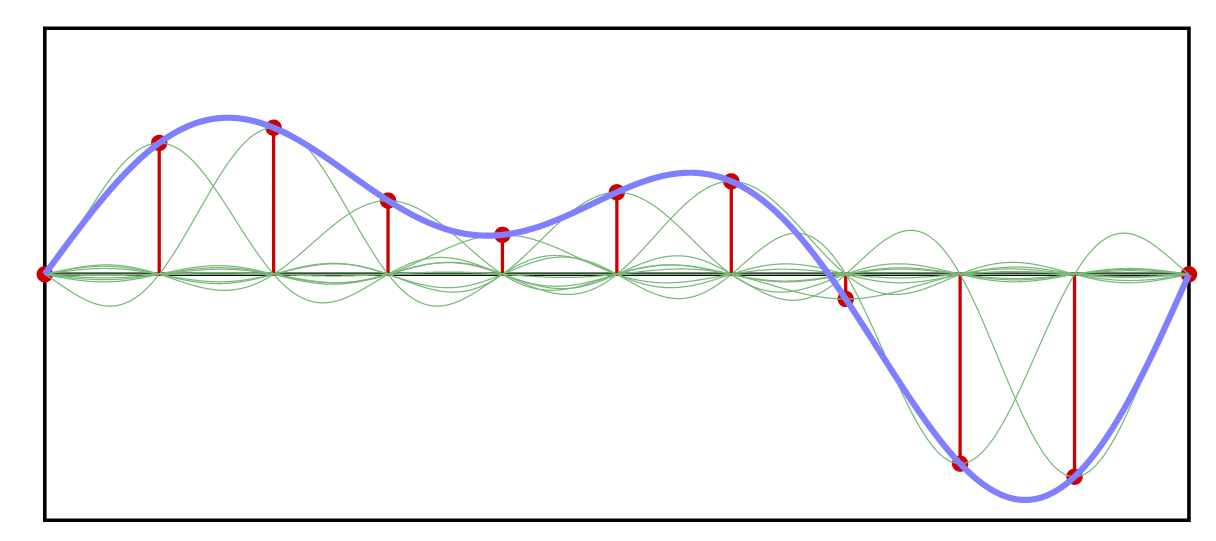
\includegraphics[scale=0.2]{images/sampling_theorem}
            \caption{Visualization of the sampling theorem}%
            \label{fig_sampling_theorem}
        \end{figure}    
   
    \item[Discrete signal] Sequence of \textbf{complex} numbers. Notation: $x[n]$. $n$ is ``a-dimensional''. Analysis $\sim$ periodic measurements and Synthesis $\sim$ stream of generated samples.
    \item[Delta signal] $x[n] = \delta[n]$. 1 when $n=0$, 0 elsewhere.
    \item[Unit step] $x[n] = u[n]$. 1 when $n \geq 0$, 0 elsewhere.
    \item[Exponential decay] $x[n] = |a|^n u[n]$ with $|a| < 1$
    \item[Signal classes] Finite-length, infinite-length, periodic, finite-support
    \item[Finite-length] Notation: $x[n], n=0,1,\ldots,N-1$. Vector: $\mathbf{x} = {[x_0,x_1,\ldots,x_{N-1}]}^T$. Good for practice.
    \item[Infinite-length] Notation: $x[n], n\in\Z$. Abstraction $\to$ good for theory.
    \item[Periodic] N-periodic sequence $\tilde{x}[n] = \tilde{x}[n+kN],\quad k,n,N \in\Z$
    \item[Finite-support] $\overline{x}[n] = \left\{\begin{array}{ll}
    x[n] & \text{if} 0 \leq n < N\\
    0 & \text{otherwise}
\end{array}\right.$
    \item[Operators] \uline{Scaling}: $<y[n] = \alpha{} x[n]$. \uline{Sum}: $y[n] = x[n] + z[n]$. \uline{Product}: $y[n] = x[n]\cdot z[n]$. \uline{Shift by $k$} (delay): $y[n] = x[n-k]$
    \item[Finite-length shift] We must chose either to use \textit{finite-support} (0's outside of the interval, shifting ``creates'' 0's) or \textit{periodic extension} (leaving on a sides makes entering on the other).
    \item[Energy] 
        \begin{equation}
            E_x = \somme{\infty}{n=-\infty}|x[n]|^2
        \end{equation}
        Infinite for periodic signals
    \item[Power] For periodic signals: $P_{\tilde{x}} \equiv \frac{1}{N}\somme{N-1}{n=0}|\tilde{x}[n]|^2$
        \begin{equation}
            P_x = \limite{N\to\infty} \frac{1}{2N+1}\somme{N}{n=-N}|x[n]|^2
        \end{equation}
    \item[Legos] DPS is composed of fundamental building blocks. See figure~\ref{dsp_legos}.
        \begin{figure}
            \centering
            \begin{subfigure}{0.45\textwidth}
                \centering
                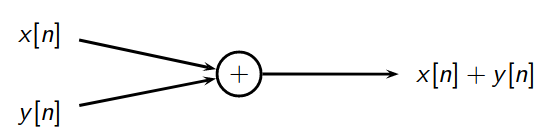
\includegraphics[scale=0.3]{images/lego_adder}%
                \label{subfig_adder}
                \caption{Adder}
            \end{subfigure}
            \begin{subfigure}{0.45\textwidth}
                \centering
                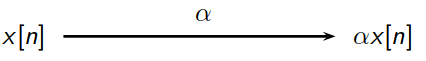
\includegraphics[scale=0.3]{images/lego_multi}%
                \label{subfig_multi}
                \caption{Multiplier}
            \end{subfigure}\\
            \begin{subfigure}{0.4\textwidth}
                \centering
                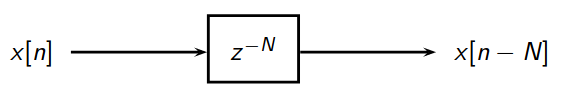
\includegraphics[scale=0.3]{images/lego_delay}%
                \label{subfig_delay}
                \caption{N-delay}
            \end{subfigure}
            \begin{subfigure}{0.45\textwidth}
                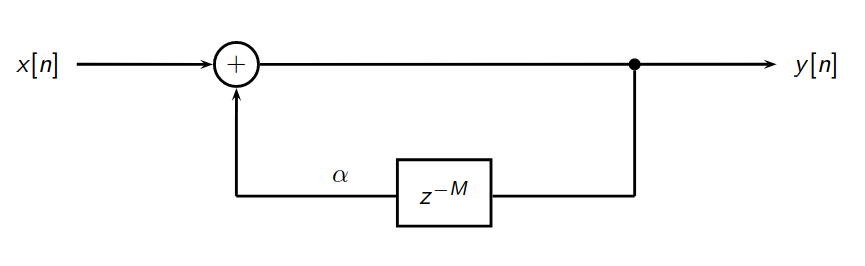
\includegraphics[scale=0.2]{images/loops}%
                \caption{A looping system}%
                \label{subfig_loop}
            \end{subfigure}  
            \caption{Fundamental building blocks}%          
            \label{dsp_legos}
        \end{figure}
  
    \item[Averages] Simple average: $m = \frac{a+b}{2}$. Moving average: take a ``local'' average 
        \begin{equation}
            y[n] = \frac{x[n] + x[n-1]}{2}
        \end{equation}
    \item[Loops]When feeding the output of a system to the input, we obtain a loop, of the type $y[n] = \alpha y[n-M] + x[n]$. This is a powerful concept! Figure~\ref{subfig_loop} shows an example. The parameters we can tweak: $M$ (size of delay), $\alpha$ (decay factor), $\overline{x}[n]$ (input signal)     
    \item[Karplus-Strong]\todo{}
\end{itemize}

%%%%%%%%%%%%%%%%%%%%%%%%
%%%% Vector space %%%%%%
%%%%%%%%%%%%%%%%%%%%%%%%
\section{Vector spaces}
\begin{itemize}
    \item[Signal model]We work in $\C^N$: vector space  of ordered tuples of $N$ complex values. $N$ can be $\infty$. We need more than a vector space, we need a \textit{Hilbert space}.
    \item[Some spaces] $\ell_2(\Z)$: space of square-summable infinite sequences. $L_2([a,b])$: space of square-integrable functions over an interval
    \item[Vector spaces]Ingredients: the set of vectors $V$, and a set of scalars (say \C). We need at least to be able to: resize vectors (multiply vector by scalar) and combine vectors together (sum them).
    \item[Formal Properties]For $\mathbf{x},\mathbf{y},\mathbf{z} \in V$ and $\alpha,\beta \in \C$:

        \begin{multicols}{2}
            \begin{itemize}[font=\normalfont, nolistsep]
                \item $\mathbf{x}+\mathbf{y} = \mathbf{y}+\mathbf{x}$
                \item $(\mathbf{x}+\mathbf{y}) + \mathbf{z} = \mathbf{x}+(\mathbf{x}+\mathbf{y})$
                \item $\alpha(\mathbf{x}+\mathbf{y}) = \alpha\mathbf{x} + \alpha\mathbf{y}$
                \item $(\alpha+ \beta)\mathbf{x} = \alpha\mathbf{x} + \beta\mathbf{x}$
                \item $\alpha(\beta\mathbf{x}) = (\alpha\beta)\mathbf{x}$
                \item $\exists 0 \in V | \mathbf{x} + 0 = 0+\mathbf{x} = \mathbf{x}$
                \item $\forall \mathbf{x} \in V \exists(-\mathbf{x}) | x+(- \mathbf{x}) = 0$
            \end{itemize}
        \end{multicols}
    \item[Dot Product]We also need something to measure and compare: \textbf{inner product} (or \textbf{dot product}). Notation: 
        \[\langle\cdot,\cdot\rangle : V\times V \to \C\]
        Measures similarity between vectors. If 0, then vectors are completely orthogonal.
    \item[Formal Properties]The dot product has several interesting properties. For $\mathbf{x},\mathbf{y},\mathbf{z} \in V$ and $\alpha\in\C$:
    \begin{multicols}{2}
        \begin{itemize}
            \item $\langle\mathbf{x}+\mathbf{y},\mathbf{z}\rangle = \langle\mathbf{x},\mathbf{z}\rangle + \langle\mathbf{y},\mathbf{z}\rangle$
            \item $\langle\mathbf{x},\mathbf{y}\rangle = \langle\mathbf{y},\mathbf{x}\rangle^*$
            \item $\langle\alpha\mathbf{x},\mathbf{y}\rangle = \alpha^*\langle\mathbf{x},\mathbf{y}\rangle$\\
            $\langle\mathbf{x},\alpha\mathbf{y}\rangle = \alpha\langle\mathbf{x},\mathbf{y}\rangle$
            \item $\langle\mathbf{x},\mathbf{x}\rangle = ||\mathbf{x}||^2 \geq 0$
            \item $\langle\mathbf{x},\mathbf{x}\rangle = 0 \iff \mathbf{x} = \mathbf{0}$
            \item If $\langle\mathbf{x},\mathbf{y}\rangle = 0$ and $\mathbf{x,y} \neq \mathbf{0}$ then $\mathbf{x}$ and $\mathbf{y}$ are orthogonal
        \end{itemize}
    \end{multicols}
    \item[Examples] In $\R^2$, the norm is simply $x_0y_0 + x_1y_1 = ||\mathbf{x}||\ ||\mathbf{y}|| \cos\alpha$. Another more interesting example, is $L_2[a,b]$ In this case, the inner product is defined as $\int_a^b x(t)y(t)\deriv{t}$
    \item[Distance]Inner product defines a norm: $||\mathbf{x}|| = \sqrt{\langle\mathbf{x},\mathbf{x}\rangle}$ while norm defines a distance: $d(\mathbf{x},\mathbf{y}) = ||\mathbf{x}- \mathbf{y}||$. In $L_2$, the distance corresponds to the Mean Square Error
    \item[For signals] the inner product is defined as following:
    \begin{equation}
        \langle\mathbf{x},\mathbf{y}\rangle = \somme{N-1}{n=0}x^*[n]y[n]
    \end{equation}
    It is well defined for all finite-length vectors in $\C^N$. Careful: if $N = \infty$, then the sum may explode! We require the sequences to be \textit{square-summable}, i.e. $\sum|x[n]| < \infty$. That is the space $\ell_2(\Z)$.
\end{itemize}

\subsection{Basis}
\begin{itemize}
    \item[Basis]Vectors can be linearly combined in vector space: $\mathbf{g} = \alpha \mathbf{x} + \beta \mathbf{y}$. A basis is a set of vectors $\{\mathbf{w}^{(k)}\}$ that lets us write any vector as a linear combination of those vectors. Alternatively, it is a set $\{\mathbf{w}^{(k)}\}$ such as there exists (unique) $\alpha_1,\alpha_2$ such as for any $\mathbf{x}$, we have \begin{equation}
        \begin{bmatrix}
            x_1\\x_2\\\vdots\\x_N
        \end{bmatrix} 
        =\alpha_1 \mathbf{w}^{(1)} + \alpha_2 \mathbf{w}^{(2)} + \ldots \alpha_k \mathbf{w}^{(k)}= \somme{N}{k=0}\alpha_k \mathbf{w}^{(k)},\quad \alpha_k \in \C%
        \label{equ_basis}
\end{equation}
    \item[Example]The canonical $\R^2$ basis is as follows: 
    $\begin{bmatrix}
        x_1\\x_2
    \end{bmatrix} =
    x_1 \begin{bmatrix}
        1\\0
    \end{bmatrix} + 
    x_2
    \begin{bmatrix}
    0\\1
\end{bmatrix}$. But this is not the \textit{only} base of $\R^2$! For example $\left\{\begin{bmatrix}
    1\\0
\end{bmatrix},\ \begin{bmatrix}
    1\\1
\end{bmatrix}\right\}$ is another valid base. Oppositely, $\left\{\begin{bmatrix}
    1\\0
\end{bmatrix},\ \begin{bmatrix}
    -1\\0
\end{bmatrix}\right\}$ is not a valid base as we can't express any vector $\mathbf{x}$ with them (e.g.\ no vector with $x_2 \neq 0$ can be expressed)
    \item[Ortho* basis]Ortho\textbf{gonal} basis: All vectors are orthogonal with one another:
    \[\langle\mathbf{w}^{(k)},\mathbf{w}^{(n)}\rangle = 0,\ \text{for } k\neq n \]
    Ortho\textbf{normal} basis same as orthogonal, but vectors are normalized; thus all are orthogonal and vectors have unit length: 
    \[\langle\mathbf{w}^{(k)},\mathbf{w}^{(n)}\rangle = \delta[n-k]\]
    \item[Basis expansion]Given a basis and a vector, finding the $\alpha_k$ might be hard. With orthonormal basis, it is easy: 
        \begin{equation}
            \alpha_k = \langle\mathbf{w}^{(k)}, \mathbf{x}\rangle
            \label{equ_basis expansion}
        \end{equation}
    \item[Basis change]We want to easily change between our basis and a given other basis:
    \[\mathbf{x} = \somme{K-1}{k=0}\alpha_k \mathbf{w}^{(k)} = \somme{K-1}{k=0}\beta_k \mathbf{v}^{(k)}\]
    We look for the $\beta_k$ using $\alpha_k, \mathbf{v}^{(k)}, \mathbf{w}^{(k)}$. Simply:
\end{itemize}
\begin{equation}
    \beta_h  = \somme{K-1}{k=0}\alpha_k \langle\mathbf{v}^{(h)}, \mathbf{w}^{(k)}\rangle = \somme{K-1}{k=0}\alpha_k c_{hk} = 
    \begin{bmatrix}
        c_{00}  &\cdots& c_{0(K-1)}\\
        & & \vdots\\
        c_{(K-1)0} & \cdots & c_{(K-1)(K-1)}
    \end{bmatrix}
    \begin{bmatrix}
        \alpha_0\\\vdots\\\alpha_{K-1}
    \end{bmatrix}
    \label{equ_basis change}
\end{equation}
\begin{itemize}


    \item[Energy]$||\mathbf{x}|| = \langle\mathbf{x},\mathbf{x}\rangle = \somme{K-1}{k=0}|x_k|^2$
    \item[Parseval]``\textit{Energy is conserved across a change of basis}
\end{itemize}
\subsection{Subspaces and approximation}
\begin{itemize}
    \item[Subspace] A vector subspace is a subset of vectors \textit{closed} under addition and scalar multiplicat0ion. 
    \item[Approximation]For a vector $\mathbf{x} \in V$ and a subspace $S \subseteq V$ then we can approximate $\mathbf{x}$ with $\hat{\mathbf{x}} \in S$.
    \item[LS]Least-square approximation. Given an orthonormal basis for $S$: ${\{\mathbf{s}^{(k)}\}}_{k=0,1,\ldots,K-1}$. Then the orthogonal projection is the ``best'' approximation over $S$. Best because it has the minimum-norm error: $\arg\min\limits_{\mathbf{y} \in S} ||\mathbf{x}- \mathbf{y}|| = \hat{\mathbf{x}}$. Beside, the error is orthogonal to approximation: $\langle\mathbf{x}-\hat{\mathbf{x}},\mathbf{x}\rangle = 0$
    \item[Gram-Schmidt]Used to build an orthonormal $\{\mathbf{u}^{(k)}\}$ set from any set $\{\mathbf{s}^{(k)}\}$. The algorithmic procedure: 
        \begin{enumerate}
            \item $\mathbf{p}^{(k)} = \mathbf{s}^{(k)} - \somme{k-1}{n=0}\langle\mathbf{u}^{(n)},\mathbf{s}^{(k)}\rangle\mathbf{u}^{(n)}$
            \item $\mathbf{u}^{(k)} = \frac{\mathbf{p}^{(k)}}{||\mathbf{p}^{(k)}||}$
        \end{enumerate}
    \item[Legendre]Legendre polynomials are a better (orthonormal) base than classical polynomials base. When approximating sinusoid with polynomials, Legendre polynomials yield a smaller error than regular polynomials base.
\end{itemize}

\subsection{Hilbert space}
\begin{itemize}
    \item[Ingredients]For a Hilbert space, we need a vector space $H(V,\C)$, an inner product $\langle\cdot,\cdot\rangle : V \times V \to \C$ and completeness
    \item[Completeness]Limiting operations must yield elements in the vector space.
\end{itemize}

%%%%%%%%%%%%%%%%%%%%%%%%
%%%%%%% Fourier %%%%%%%%
%%%%%%%%%%%%%%%%%%%%%%%%
\section{Fourier}
\subsection{Introduction}
\begin{itemize}
    \item[Time domain]Discrete signals are expressed as linear combinations of ``atomic'' time units
    \[x[n] = \somme{N-1}{k=0}x[k]\delta[n-k] \iff \mathbf{x} = \somme{N-1}{k=0}x_k \boldsymbol{\delta}^k\]
    Where $\{\boldsymbol{\delta}\}$ is a canonical basis for $\C^N$, e.g. $\boldsymbol{\delta}^{(2)} = [0\ 0\ 1\ 0\ \cdots\ 0]$
    \item[Frequency domain] \uline{Fourier analysis}: express a signal as combination of periodic oscillations:
        \begin{equation}
            \mathbf{x} = \somme{N-1}{k=0} X_k \mathbf{w}^{(k)}
        \end{equation}
        with $\mathbf{w}^{(k)}$ the Fourier basis. The \uline{Fourier transform} is a change of basis in the space of discrete time signals.
    \item[Analysis/Synthesis] 
        \textit{Fourier analysis}: time domain $\to$ frequency domain, to find contribution of different frequencies.\\
        \textit{Fourier synthesis}: frequency domain $\to$ time domain, to create signals with known frequency content.
    \item[Math reminders] $e^{j\alpha} = \cos\alpha + j\sin\alpha \simeq$ point on the unit circle, at angle $\alpha$. See Figure\ref{fig_trigo circle}.
        \begin{figure}
            \centering
            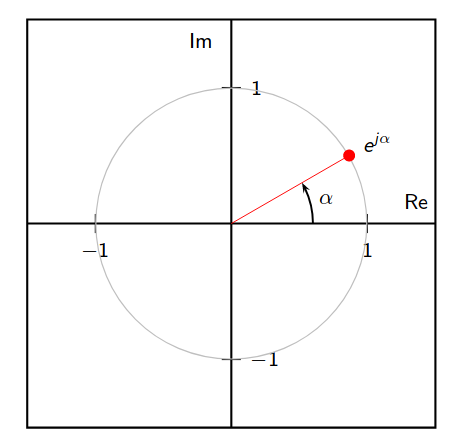
\includegraphics[scale=0.4]{images/trigo_circle}
            \caption{The trigonometric circle}%
            \label{fig_trigo circle}
        \end{figure}
        Rotations of an angle $\beta$ (centre at origin) are made by multiplying by $e^{j\beta}$. To represent discrete-time oscillatory, we need a frequency $\omega$, an initial phase $\phi$ and an amplitude $A$:
        \[x[n] = Ae^{j(\omega n + \phi)} = A[\cos(\omega n + \phi) + j\sin(\omega n+ \phi)]\]
    \item[Periodicity] Consider the signal $x[n] = e^{j\omega n}$, then $x[n+1] = e^{j\omega n} x[n]$. In some cases, this is periodic. The condition for $e^{j\omega n}$ to be periodic in $n$, is to have $\omega = \frac{M}{N}2\pi$ with $M,N \in \Z$. So if the frequency is a (rational) multiple of 2$\pi$, the signal is periodic.
    \item[Max Frequency]The higher we chose $\omega$, the `less points'' we will have between each loop. But once we reached $\omega = \pi$, we only have 2 points ($\pm 1$). Going at speed $\pi+\alpha$ is similar as going at speed $-(\pi-\alpha)$
    \item[Digit./Physic.\ freq]In discrete time, $n$ is a-dimensional, just a counter. Periodicity is the number of samples before pattern repeats. But in real world, periodicity is the number of \textit{seconds} before pattern repeats; it's measured in $Hz\ (s^{-1})$. Now, set $T_s$ seconds between samples, and a periodicity of $M$ samples (that is a periodicity of $MT_s$ seconds). Then the real-world frequency is $\frac{1}{MT_s}$
\end{itemize}
\subsection{Fourier Basis}
\begin{itemize}
    \item[Basis]The set of $N$ signals in $\C^N$ represented in eq.~\ref{equ_fourier basis} is an orthogonal basis in $C^N$. The proof won't be presented here. Note that the vectors are \uline{not} orthonormal. The normalization factor would be $1/\sqrt{N}$
\end{itemize}        
\begin{equation}
    w_k[n] = e^{j\frac{2\pi}{N}nk},\ n,k = 0,1,\ldots,N-1 \sim \{\mathbf{w}^{(k)}\}_{k=0,1,\ldots,N-1} \text{ with } w_n^{(k)} = e^{j\frac{2\pi}{N}nk}
    \label{equ_fourier basis}
\end{equation}
\subsection{Discrete Fourier Transform}
\begin{itemize}
    \item[Basis expansion]Following Equation~\ref{equ_basis expansion}, the \textit{analysis} formula (respectively the \textit{synthesis} formula) is
        \begin{equation}
            X_k = \langle\mathbf{w}^{(k)},\mathbf{x}\rangle \qquad \mathbf{x} = \frac{1}{N} \somme{N-1}{k=0}X_k \mathbf{w}^{(k)}
        \end{equation}
    \item[Change of basis]We try to define the matrix of basis change (as in Equation~\ref{equ_basis change}). First we define $W_N = e^{-j\frac{2\pi}{n}}$ (or $W$ when $N$ is evident). Then the change of basis matrix $\mathbf{W}$ with $\mathbf{W}[n,m] = W_N^{nm}$: 
        \begin{equation}
            W = 
            \begin{bmatrix}
                1 & 1 & 1 & 1 & \cdots & 1\\
                1 & W^1 & W^2 & W^3 & \cdots & W^{N-1}\\
                1 & W^2 & W^4 & W^6 & \cdots & W^{2(N-1)}\\
                & & & \vdots\\
                1 & W^{N-1} & W^{2(N-1)} & W^{3(N-1)} & \cdots & W^{(N-1)^2}
            \end{bmatrix}
        \end{equation}
\end{itemize}
\end{document}